
% \subsection{The Quadratic Assignment Problem} {
%
% }

The Quadratic Assignment Problem (QAP) was introduced by \citet{Koopmans:1957gf}, motivated by the problem of optimally assigning manufacturing plants to locations in a way that maximises total revenue.
The given a matrix of revenues that plants will generate in different locations, a matrix of distances between the locations, and a `flow' matrix containing the quantity of commodity bundles that must be transported between plants per time unit.

More formally, the matrix \([r_{ki}]\) contains the known revenue each plant \(k\) will have a when placed at location \(i\).
The matrix \([a_{kl}]\) contains the required commodity flow between plant \(k\) and plant \(l\), and the matrix \([b_{ij}]\) contains the cost of transport per unit flow between location \(i\) and location \(j\). These are often referred to as the flow matrix and the distance matrix, respectively.
The problem is then to find a permutation \(\pi^{*} \in S_n\) (\(S_n\) is the symmetric group of order \(n\)) that maximises the total revenue:

\[ \pi^{*} = \max_{\pi} \left(\sum_{k}{r_{k\pi(k)}} - \sum_{k}\sum_{l}{a_{kl}b_{\pi(k)\pi(l)}}\right) \]

where  \(\pi(k) = i\) indicates that plant \(k\) is to be placed at location \(i\).

Many authors ignore the linear term \(\sum_{k}{r_{k\pi(k)}}\), both because it is not necessary in some applications, and because it does not significantly increase the difficulty of the problem. For this reason, the QAP is often expressed as a minimisation problem as presented in \eqref{eq:qap}.

\begin{equation}
    \label{eq:qap}
    \pi^{*} = \min_{\pi} \sum_{k}\sum_{l}{a_{kl}b_{\pi(k)\pi(l)}}
\end{equation}

\citeauthor{Koopmans:1957gf} established the place of the QAP as a difficult NP-Hard problem by indicating that the Travelling Salesman Problem can be expressed as a special case. The QAP has since been referred to as ``one of the most difficult problems in the NP-hard class'' \citep{Loiola:2007jk}, and has attracted much research attention due to its difficulty making it an attractive benchmark for newly developed generic optimisation algorithms and metaheuristics, due to its theoretical importance, and due to its many practical applications.
\citet{Loiola:2007jk} gives a detailed survey of approaches and applications of the QAP, referencing 365 papers published between its introduction in 1957 up until 2007. We discuss some more recent applications and solution approaches in Section~\ref{sec:applications} and Section~\ref{sec:approaches} respectively.

\subsection{Recent Applications} {
    \label{sec:applications}

	\citeauthor{Koopmans:1957gf} uses the application of optimally locating manufacturing plants to maximise revenue to motivate the QAP. This problem is sometimes called the Facilities Layout Problem (FLP), and is the most common application of the QAP \citep{Loiola:2007jk}.
	\citet{Samanta:2015hk} used the QAP in the layout optimisation of a bus body manufacturing plant.
	\citet{XiongfengFeng:2015jo} recently used the QAP to improve the layout of departments in a hospital. They were able to decrease the average walking time for outpatients by 11.55\%.

	The QAP has applications beyond instances of the FLP.
	Recently, \citep{Alguliyev:2015jw} used it in the unsupervised generation of summaries of documents.
	\citet{Azab:2015eq} applied the QAP to a problem in manufacturing that required optimisation of the sequence in which features of a product would be machined in order to minimise handling time, given a set of precedence constraints between features.

	% While the application of optimally locating manufacturing plants to maximise revenue that \citeauthor{Koopmans:1957gf} used to motivate the QAP is useful, many additional practical applications have been found since.

	% \citet{Loiola:2007jk} lists many publications that apply the QAP to practical problems, including the

	% Mention applications listed by \citet{Loiola:2007jk}.

	% Mention \citep{Bhati:2014as} in the intro, then state that specific examples follow.

}

\subsection{Current approaches} {
    \label{sec:approaches}

	% \todo{define steepest descent search}

    % Use Merz:1999kl as an example of papers that compare methods using the QAP.

    % Discuss the comparison of memory schemas used in \citet{Meneses:2011hg}.

	\citet{Meneses:2011hg} investigated the effects of different memory schemas on the performance of the memetic algorithm for the QAP described in \citet{Inostroza:2008md}.
	\citeauthor{Meneses:2011hg} uses a structured population based on a ternary tree introduced by \citet{Inostroza:2008md}. This structure is considered to be a long-term memory schema, as it is used to guide the interaction of individuals in the algorithm.
	Four other memory schemas are considered in their comparisons; Fixed Tabu List \citep{glover1989tabu}, Variable Tabu List (VTL), Reduced Search (RS), and greedy Steepest Descent search (SD).
	Steepest Descent search repeatedly improves a solution by moving to the best solution in its 2-swap neighbourhood until a local maximum is found. The greedy variant used by \citeauthor{Meneses:2011hg} simply moves to the first improving solution rather than finding the best neighbouring solution.
	Reduced Search is an SD search where the equal positions among the parents of the initial individual are initially tabu.
	The eight combinations of memory schemas are evaluated by running them on 30 selected instances of the QAP taken from the literature.
	Their best classifier combined VTL, RS, and SD and the structured population to achieve an average deviation from the best known results of 0.133\%, and their statistical tests indicated that combining memory schemas generally led to better performance of their algorithm.


	% Discuss: An implementation of the iterated tabu search algorithm for the quadratic assignment problem

	% Describe the ITS framework

	% Describe the controlled chained mutation

	\citet{Misevicius:2012dj} proposed an implementation of the Iterated Tabu Search (ITS) algorithm for the QAP.
	The ITS algorithm begins by generating a random solution and improving it using tabu search. Then, for a given number of iterations, it repeatedly applies a mutation operation to the current solution before improving it again, always saving the best solution found so far to be returned as its result. The mutation operator and intensification strategies used by ITS are intended to overcome the `stagnant behaviour' that typically occurs when using algorithms based on tabu search.

	The mutation operator used that produces a new permutation with a Hamming distance of \(\mu\) from its input. To do this it randomly generates a number of sequences of \(\mu\) transpositions, ensuring that their composition has the correct Hamming distance from \(\mu\), and ranks each sequence according to a \newterm{disruptiveness} metric. The most disruptive mutation is chosen to produce the result permutation.
	The number of sequences to generate is a parameter of the algorithm.
	The parameter \(\mu\) has an initial value \(\mu_\text{min}\) and is increased on every iteration, and reset to \(\mu_\text{min}\) whenever an improved local optimum is found or a maximum value \(\mu_\text{max}\) is reached.

	The ITS algorithm uses three intensification strategies.
	The first causes the tabu list to be ignored once every \(I_1\) iterations, allowing the best neighbouring solution to be accepted without a tabu test.
	The second strategy is to run a special `fast' SD search to improve the current solution whenever a neighbouring solution is found that improves upon the current solution. This SD search is only run if it has already been run within the last \(I_2\) iterations.
	The third strategy is to decrease all values in the tabu list by half whenever a new local optimum is encountered.

	\citeauthor{Misevicius:2012dj} tested ITS on instances from QAPLIB \citep{Burkard:1997ve}, and found new best known values for three of the problems in the library. The algorithm achieved an average deviation from the best known solutions of 55 selected problem instances of 0.5\%.

    % Describe the memetic algorithm in \citet{Harris:2015kw}.

	\todo{Make this section smoother.}
    \citet{Harris:2015kw} introduces a memetic algorithm to solve the QAP.
    Their method represents candidate solutions by simply storing the image of the permutations in an array.

    The ternary tree memory schema previously introduced in \citet{Inostroza:2008md} is used to structure the population and to guide the other stages of the algorithm.
    The population is divided into 13 nodes which form a complete ternary tree. Each node contains 6 individuals, a \newterm{current} individual, and five \newterm{pocket} individuals.
    This population structure is illustrated in Figure~\ref{fig:ternary-tree}.

	Their algorithm uses the CX recombination operator used by \citet{Merz:2000ek} as a crossover operator, followed by improvement using tabu search to generate new individuals.
	The CX operator notably does not perform any implicit mutation, in the sense that every plant assigned to a location \(i\) in the child permutation is also assigned to location \(i\) in at least one of its parents.
	In fact, \citeauthor{Harris:2015kw} do not use random mutation in their algorithm, relying instead on a randomly initialised population, and a method of randomly restarting the population whenever the current best solution has not changed for a given number of iterations. The population is restarted by removing all but the best individual before adding a randomly generated individual (improved using tabu search) to each node.

	Each iteration of the algorithm generates a new individual in each node using a crossover operator. One of the parents of the crossover is always chosen randomly from the source node, and the other parent is chosen randomly from the same node if the population diversity is high, or from a random node from a different subpopulation of the ternary tree if the population's diversity is low. This strategy is intended to prevent rapid diversity loss. Four simple rules are used to determine whether and how the new individual should be incorporated into the node's set of pocket solutions. These rules are also designed to reduce the loss of diversity.

	The algorithm presented by \citeauthor{Harris:2015kw} was tested on the complete QAPLIB set of problems and achieved an average gap of 0.049\% below the best known solutions when run with a time limit of 5 minutes. The average time before the best solution was found was 3.93 seconds.

	\begin{figure}
		\centering
		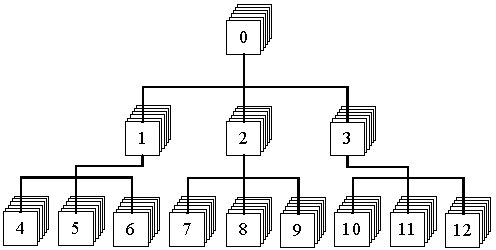
\includegraphics[width=0.5\textwidth]{resources/ternary-tree.pdf}%
		\caption{The ternary tree population introduced in \citet{Inostroza:2008md}, consisting of 13 nodes each containing a single \newterm{current} individual, and five \newterm{pocket} individuals.}
		\label{fig:ternary-tree}
	\end{figure}


    % BMA \citet{Benlic:2015gp}.

	\citet{Benlic:2015gp} proposed a new memetic algorithm for the QAP called BMA, which uses Breakout Local Search (BLS) as its local search procedure, the CX crossover operator used by \citet{Merz:2000ek}, a fitness-based population replacement strategy, and an adaptive mutation mechanism.

	BMA first randomly generates an initial population \(P\), before improving each individual using BLS.
	BLS is a local search procedure that improves a solution by first performing a steepest descent search using the full 2-swap neighbourhood, before applying \(L\) \newterm{peturbation moves} intended to diversify the search. These moves amount to either \(L\) iterations of tabu search, or the application of \(L\) random transpositions to the current solution permutation. The choice of random or tabu search moves is probabilistic, and is based on the number of consecutive non-improving solutions found by the SD search. \(L\) is set to an initial value \(L_0\) plus the number of consecutive visits the SD search has made to the immediate previous local optimum.
	The BLS search consists of a fixed number of iterations of SD search followed by perturbation moves, and then a final SD search.
	\citeauthor{Benlic:2015gp} use the BLS-QAP algorithm presented in \citet{Benlic:2013gi}.

	Then in each generation, a subset \(p \subset P\) of \(|p|\) parent individuals are chosen from the population, by repeatedly randomly selecting \(\lambda\) individuals from \(P\) and adding the best of them into \(p\) if it is not already present in \(p\).
	Two random parents from the set \(p\) are selected for crossover using the CX crossover operator used by \citet{Merz:2000ek} to produce a new individual. % \(pi^0\).
	The new individual is improved using BLS, before being subjected to a replacement strategy to determine whether it should be included into the population. The replacement strategy simply replaces the worst solution in the population with the new solution as long as the new solution is better than the worst solution, and the new solution is not identical to any existing solution in the population.

	If the best solution found is not improved after \(v\) generations, then a mutation procedure is performed on each individual in the population. The mutation operation produces a random permutation with a Hamming distance of \(\mu\) from its input, where \(\mu\) is chosen to be proportional to the number of iterations since the last improvement to the best solution less \(v\).

	BMA was able to achieve an average gap of 0.016\% below the best known solutions among all problems in QAPLIB within a time limit of 30 minutes, and was able to find the best known solution within 2.5 minutes for all but the 21 `hardest' instances.


	% TBH-PSO \citep{Helal:2015de}

	\citet{Helal:2015de} presents variations of an algorithm called TBH-PSO, which combines Hierarchical Particle Swarm Optimisation (HPSO) and Tabu Local Search to solve to QAP.

	HPSO is a metaheuristic that maintains a population of `particles' each comprised of a state and a velocity. Each particle's state represents a candidate solution to the problem being solved, and each velocity influences the way that the particle moves through the solution space.
	The implementation of HPSO presented by \citeauthor{Helal:2015de} arranges the particles in a ternary tree structure similar to that of \citet{Harris:2015kw}, except that each node in the tree consists of a single particle.
	In each iteration of the algorithm, the velocity of each particle is updated using a function of its state, the state of its parent, the best states ever attained by itself and its parent, and its current depth in the hierarchy.
	The velocity components are then clamped between constant minimum and maximum values, and the state is recalculated from the velocity.
	Following the state-velocity update the value of each particle is compared to its immediate children, and if the value of the best child is better than the current particle's value, the two particles positions in the tree are swapped.

	TBH-PSO applies PSO to the QAP by representing the velocity of each particle as an \(n \times n\) matrix \([v_{i}]\) in which each \(v_{iyz}\) represents the tendency of particle \(i\) to assign plant \(y\) to location \(z\).
	The algorithm defines a stochastic procedure to generate a particle's state from its velocity, which is run whenever a particle's velocity changes.

	Tabu Search is used to improve the root particle in the hierarchy after each iteration of PSO.

	\citeauthor{Helal:2015de} ran TBH-PSO on 31 selected instances from QAPLIB, and achieved an average deviation from the best known solutions of 0.0919\%, with an average running time of 44 seconds.
}
